\documentclass[crop,tikz]{standalone}
\usepackage{pgfplots}
\usepackage{tikz-3dplot}
\begin{document}

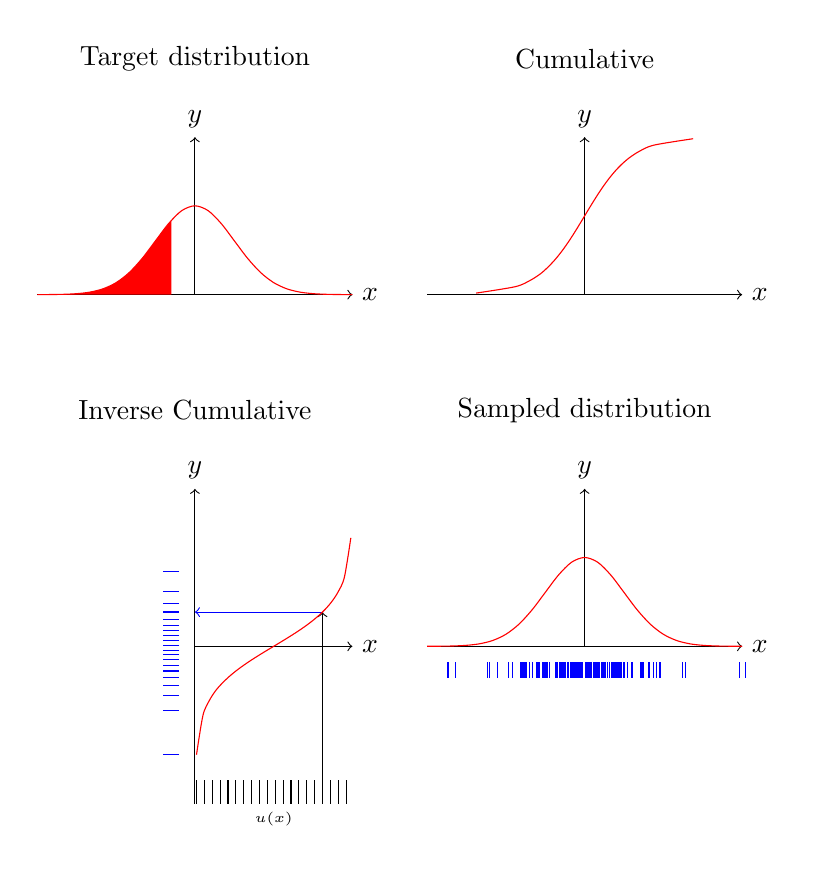
\begin{tikzpicture}[
  declare function={normal(\x,\m,\s)=1/(2*\s*sqrt(pi))*exp(-(\x-\m)^2/(2*\s^2));},
  declare function={erf(\x)=%
      (1+(e^(-(\x*\x))*(-265.057+abs(\x)*(-135.065+abs(\x)%
      *(-59.646+(-6.84727-0.777889*abs(\x))*abs(\x)))))%
      /(3.05259+abs(\x))^5)*(\x>0?1:-1);},
  declare function={cdfnormal(\x)=0.5*(1+erf((\x-1)/(sqrt(2))));},
  declare function={invnormal(\x)=0.3*ln(\x/(1-\x));}, % aprox. using logit(x)
  ]
\matrix[column sep=5mm, row sep=10mm] {
\begin{scope}[yscale=2]
  \draw[->] (-2,0) -- (2,0) node[right] {$x$};
  \draw[->] (0,0) -- (0,1) node[above] {$y$};
  \draw[domain=-2:2,smooth,variable=\x,red] plot (\x,{normal(\x,0,0.5)});
  \fill[fill=red] (-2,0) -- plot [domain=-2:-0.3] (\x,{normal(\x,0,0.5)}) -- (-0.3,0) -- cycle;
  \node [black] at (0, 1.5) {Target distribution};
\end{scope}
&
\begin{scope}[yscale=2]
  \draw[->] (-2,0) -- (2,0) node[right] {$x$};
  \draw[->] (0,0) -- (0,1) node[above] {$y$};
  \draw[domain=0.01:0.99,smooth,variable=\x,red] plot ({invnormal(\x)},\x);
  \node [black] at (0, 1.5) {Cumulative};
\end{scope}
\\
\begin{scope}[xscale=2]
  \draw[->] (0,0) -- (1,0) node[right] {$x$};
  \draw[->] (0,-2) -- (0,2) node[above] {$y$};
  \foreach \i in {0.01,0.06,...,0.99} {
    \draw[black] (\i,-2) -- (\i,-1.7);
    \draw[blue] (-0.1,{invnormal(\i)}) -- (-0.2,{invnormal(\i)});
  }
  \def\xref{0.81}
  \draw[->, black] (\xref,-1.7) -- (\xref,{invnormal(\xref)});
  \draw[->, blue] (\xref,{invnormal(\xref)}) -- (0,{invnormal(\xref)});
  \draw[domain=0.01:0.99,smooth,variable=\x,red] plot ({\x},{invnormal(\x)});
  \node [black] at (0, 3) {Inverse Cumulative};
  \node [black] at (0.5, -2.2) {\tiny $u(x)$};
\end{scope}
&
\begin{scope}[yscale=2]
  \draw[->] (-2,0) -- (2,0) node[right] {$x$};
  \draw[->] (0,0) -- (0,1) node[above] {$y$};
  \foreach \i in {1,2,...,150} {
    \pgfmathsetmacro{\t}{0.5+0.5*rand}
    \draw[blue] ({invnormal(\t)},-0.1) -- ({invnormal(\t)},-0.2);
  }
  \draw[domain=-2:2,smooth,variable=\x,red] plot (\x,{normal(\x,0,0.5)});
  \node [black] at (0, 1.5) {Sampled distribution};
\end{scope}
\\
};
\end{tikzpicture}

\end{document}